\section{EXPERIMENTS} \label{sec:experiments}

In this section we present numerical results of the validation benchmark and
  discuss a proof of concept application in the domain of particle
  accelerators.

\subsection{Optimizer Validation}

\begin{figure}
    \centering
    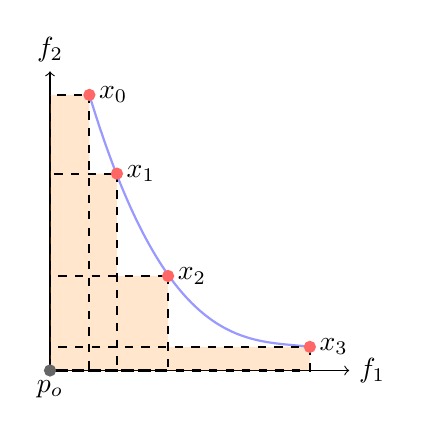
\begin{tikzpicture}[text=black]
      \coordinate (y) at (0,3.8);
\coordinate (x) at (3.8,0);
\draw[<->] (y) node[above] {$f_2$} -- (0,0) --  (x) node[right]
{$f_1$};

\path
  coordinate (start) at (0.5,3.5)
  coordinate (c1) at +(1.5,0.2)
  coordinate (c2) at +(2.5,0.4)
  coordinate (top) at (3.3,0.3);

\draw [thick, blue!40!white] (start) .. controls (c1) and (c2) .. (top);
(start) .. controls (c1) and (c2) .. (top) -- (3.3,0.0);
%\draw [fill, color=blue, draw opacity=0, fill opacity=0.2] (0,0) -- (0.0, 3.5) --
%(start) .. controls (c1) and (c2) .. (top) -- (3.3,0.0);


\draw[fill, color=orange, draw opacity=0, fill opacity=0.2] (0,0) -- (0, 3.5) --
(start) -- (0.5,2.5) -- (0.85, 2.5) -- (0.85, 1.2) -- (1.5, 1.2) -- (1.5, 0.3) -- (top) -- (3.3, 0.0);
\draw[dashed, thick] (start) rectangle (0,0);
\draw[dashed, thick] (top) rectangle (0,0);
\draw[dashed, thick] (0.85,2.5) rectangle (0,0);
\draw[dashed, thick] (1.5,1.2) rectangle (0,0);

\filldraw [red!60!white]
(start) circle (2pt) node[right, black] {$x_0$}
(0.85,2.5) circle (2pt) node[right, black] {$x_1$}
(1.5,1.2) circle (2pt) node[right, black] {$x_2$}
(top) circle (2pt) node[right, black] {$x_3$};

\filldraw [black!60!white]
(0,0) circle (2pt) node[below, black] {$p_o$};


    \end{tikzpicture}
  \caption{The hypervolume for a two-objective optimization problem
  corresponds to the shaded area formed by the dashed rectangles spanned by
  all points on the Pareto front and an arbitrary selected origin $p_o$.}
  \label{fig:hypervolume}
\end{figure}

To ensure that the optimizer works correctly we solved the benchmark
  problem (\ref{eqn:bench}).
To that end, we use a metric for comparing the quality of a Pareto
  front.
Given a point in the Pareto set, we compute the $m$ dimensional volume (for
  $m$ objectives) of the dominated space, relative a chosen origin.
We visualize this for $2$ objectives in Figure~\ref{fig:hypervolume}.
For further information and details of the implementation see~\cite{whbb:12}.
Figure~\ref{fig:pisa_bench} and the corresponding hypervolume values in
  Table~\ref{tbl:bench_rms_error}.
The reference Pareto front is clearly very well approximated.
It took a total of 1100 function evaluations to perform this computation.
The hypervolume of the reference solution ($0.6575$) for our benchmark was
  computed by sampling the solution provided in~\cite{hbwh:05}.

\begin{figure}
  \centering
    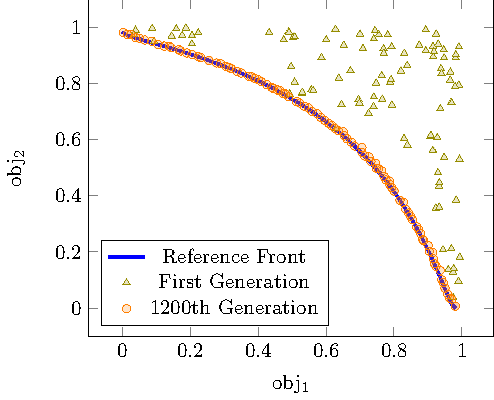
\includegraphics[width=0.7\linewidth]{figures/valid_front}
  \caption{Variator benchmark after $1100$ function evaluations using binary
           crossover and independent gene mutations (each gene mutates with
           probability $p=\frac{1}{2}$) on a population of $100$
           individuals.}
  \label{fig:pisa_bench}
\end{figure}

\begin{table}%[h!]
\begin{center}
  \caption{Convergence of benchmark problem with errors relative to
    hypervolume of sampled reference solution.}
  \label{tbl:bench_rms_error}
  \begin{tabular}{lcc}
    \hline\noalign{\smallskip}
    tot.\ function  & hyper volume & relative error\\
    evaluations    & & \\
    \noalign{\smallskip}\hline\noalign{\smallskip}
    100  &  0.859753 & $3.076 \times 10^{-1}$ \\
    \noalign{\smallskip}\hline\noalign{\smallskip}
    200  &  0.784943 & $1.938 \times 10^{-1}$ \\
    500  &  0.685183 & $4.210 \times 10^{-2}$ \\
    900  &  0.661898 & $6.689 \times 10^{-3}$ \\
    1100 &  0.657615 & $1.749 \times 10^{-4}$ \\
    \noalign{\smallskip}\hline
  \end{tabular}
\end{center}
\end{table}

From Table~\ref{tbl:bench_rms_error} we deduce that we achieved satisfactory
  convergence to the sampled reference Pareto front after 1000 (plus the
  additional 100 evaluations for the initial population) function evaluations.


\subsection{Ferrario Matching Point}\label{ferrario}

As a verification and proof of concept we reproduce the Ferrario
  matching point discovered by Ferrario \textit{et~al.}~\cite{fcpr:00},
  by formulating the problem as a  multi-objective optimization problem.
Using the low-dimensional and fast nature of their new simulation code
  Homdyn~\cite{homdyn}, an extensive beam dynamics study was conducted.

One of the results of the study presented in \cite{fcpr:00} was the discovery
  of a novel working point.
The authors noticed that the second emittance minimum can profit from the
  additional emittance compensation in the accelerating traveling wave
  structure ensuring that the second emittance minimum occurs at a higher
  energy.
This property is attained if the beam emittance has a maximum and the root
  mean square (rms) beam size has a minimum at the entrance of the first
  accelerating traveling wave structure.
This behavior is illustrated in Figure~\ref{fig:fer_match}.

\begin{figure}
  \centering
  
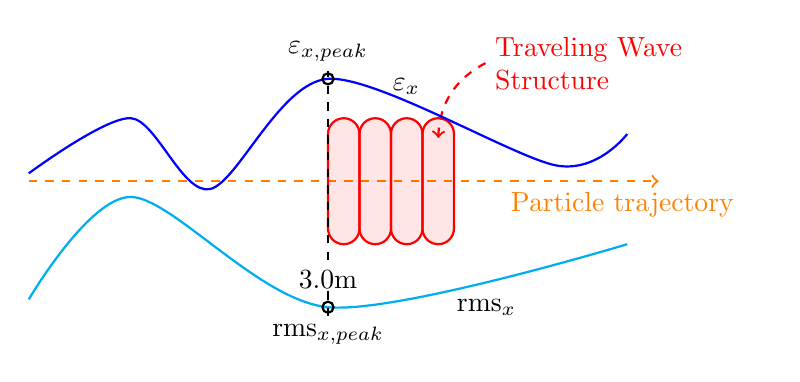
\begin{tikzpicture}

  \draw[dashed, thick, color=orange] (1.2,2.0) edge[->] (9.2,2);
  \node[orange, right, text width=3.2cm] at (7.2, 1.7) {Particle trajectory};

  %\draw[thick] (1.2,2.5) edge (9,2.5);
  %\draw[thick] (1.2,1.5) edge (9,1.5);
  %\node[above] at (1.0, 1.45) {Beam pipe};

  \draw[thick,color=red, fill=red, fill opacity=0.1, rounded corners=2mm] (5.0,1.2)
      rectangle (5.4,2.8);
  \draw[thick, dashed] (5.0,1.0) edge (5.0,3.4) node[below] {$3.0$m};
  \draw[thick,color=red, fill=red, fill opacity=0.1, rounded corners=2mm] (5.4,1.2)
      rectangle (5.8,2.8);
  \draw[thick,color=red, fill=red, fill opacity=0.1, rounded corners=2mm] (5.8,1.2)
      rectangle (6.2,2.8);
  \draw[thick,color=red, fill=red, fill opacity=0.1, rounded corners=2mm] (6.2,1.2)
      rectangle (6.6,2.8);
  \node[right, red, text width=2.8cm] at (7.0, 3.5) {Traveling Wave Structure};
  \draw[dashed, thick, color=red, bend right] (7.0,3.5) edge[->] (6.4,2.55);

  \draw[thick, cyan] plot [smooth, tension=0.5] coordinates {
      (1.2,0.5)
      (2.5,1.8)
      (5.0,0.4)
      (8.8,1.2)};
  \draw[thick, dashed] (5.0,0.6) edge (5.0,0.2);
  \draw[thick] (5.0,0.4) circle (2pt);
  \node[very thick, right] at (6.5, 0.4) {rms$_x$};
  \node[below] at (5.0, 0.3) {rms$_{x\text{, peak}}$};

  \draw[thick, blue] plot [smooth, tension=0.5] coordinates {
      (1.2,2.1)
      (2.5,2.8)
      (3.5,1.9)
      (5.0,3.3)
      (7.9,2.2)
      (8.8,2.6)};
  \draw[thick] (5.0,3.3) circle (2pt);
  \node[right] at (5.7, 3.2) {$\varepsilon_x$};
  \node[above] at (5.0, 3.4) {$\varepsilon_{x\text{, peak}}$};

\end{tikzpicture}

  \caption{Illustration of the Ferrario matching criteria: beam emittance
  attains a maximum and rms beamsize a minimum at the entrance to the first
  accelerating traveling wave structure.}
  \label{fig:fer_match}
\end{figure}

By artificially reproducing this working point as the solution of a
  multi-objective optimization problem given in equations
  (\ref{eq:swissfel:p1}) to (\ref{eq:swissfel:lastdvar}),
  we demonstrate the automation of discovering optimal beam dynamics behaviors
  given a set of desired objectives.

\begin{align}
  \text{min}  \quad & \left[ \Delta \text{rms}_{x,\text{peak}} = \vert 3.0 -
  \text{rms}_{x,\text{peak}} \vert, \right. \label{eq:swissfel:p1}\\
                    & \Delta \varepsilon_{x,\text{peak}}  = \vert 3.0 -
                    \varepsilon_{x,\text{peak}} \vert, \label{eq:swissfel:p2}\\
                    & \left. \vert \text{rms}_{x, \text{peak\_pos}} -
                    \varepsilon_{x,\text{peak\_pos}} \vert
                    \label{eq:swissfel:p3} \right]^T\\
  \text{subject to} \quad & q = 200 \left[\text{pC}\right] \label{eq:swissfel:firstconstr}\\
              \quad & \text{Volt}_{\text{RF}} = 100 \left[\text{MV/m}\right] \label{eq:swissfel:lastconstr}\\
              \quad & \sigma_{L} \leq \sigma_x = \sigma_y \leq \sigma_{U} \label{eq:swissfel:firstdvar}\\
              \quad & \text{KS}_{L} \leq \text{KS}_{\text{RF}} \leq \text{KS}_{U} \label{eq:swissfel:seconddvar}\\
              \quad & \text{LAG}_{L} \leq \text{LAG}_{\text{RF}} \leq \text{LAG}_{U} \\
              \quad & \Delta z_{L\text{KS}} \leq \Delta z_{\text{KS}} \leq \Delta z_{U\text{KS}} \label{eq:swissfel:lastdvar}
\end{align}

The first two objectives minimize the distance from the position of the current
  minimum peak to the expected peak location at $3.0$\,m for transverse bunch
  size (beam waist) and emittance (see Figure~\ref{fig:fer_match}).
The third objective (\ref{eq:swissfel:p3}) adds a condition preferring
  solutions that have their emittance and rms peak locations at the same
  $s$-coordinate.
Equations (\ref{eq:swissfel:firstconstr}) and (\ref{eq:swissfel:firstdvar})
  define constraints for initial conditions for the simulation: charge,
  gun voltage and laser spot size.
Design variables given in (\ref{eq:swissfel:seconddvar}) to
  (\ref{eq:swissfel:lastdvar}) correspond to field strengths of the
  first focusing magnet, its displacement, and the phase of the gun.

In order to compute the peaks, we employed an additional Python script.
This script was called in the \textsc{OPAL}~input file, after the simulation
  finished using the \texttt{SYSTEM} functionality.
Once the peaks (in a given range) were located, the two objectives
  (\ref{eq:swissfel:p1}) and (\ref{eq:swissfel:p2}) were computed and their
  values written into corresponding files.
The custom \texttt{fromFile} functor allows us to access the values stored in
  the peak finder Python script result files

\vspace{0.2cm}
{\footnotesize \begin{verbatim}
    rmsx:  OBJECTIVE, EXPR="statVariableAt("rms_x-err.dat", "var")";
    emitx: OBJECTIVE, EXPR="statVariableAt("emit_x-err.dat", "var")";
    match: OBJECTIVE, EXPR="fabs(statVariableAt("emit_x-peak.dat", "var") -
                                 statVariableAt("rms_x-peak.dat", "var"))";
\end{verbatim}}
\vspace{0.2cm}

\noindent
The design variables and the assembly of the multi-objective optimization problem
  can be included in the \textsc{OPAL}~input file as shown below:

\vspace{0.2cm}
{\footnotesize \begin{verbatim}
    d1:  DVAR, VARIABLE="SIGX", LOWERBOUND="0.00025", UPPERBOUND="0.00029";
    d2:  DVAR, VARIABLE="FIND1_MSOL10_i", LOWERBOUND="110", UPPERBOUND="120";
    d3:  DVAR, VARIABLE="D_LAG_RGUN", LOWERBOUND="-0.1", UPPERBOUND="0.1";
    d4:  DVAR, VARIABLE="D_SOLPOS", LOWERBOUND="-0.05", UPPERBOUND="0.05";

    objs:    OBJECTIVES = (rmsx, emitx);
    dvars:   DVARS = (d1, d2, d3, d4);
    constrs: CONSTRAINTS = ();
    opt:     OPTIMIZE, OBJECTIVES=objs, DVARS=dvars,
             CONSTRAINTS=constrs;
\end{verbatim}}
\vspace{0.2cm}

All numerical experiments in this sections were executed on the
  \textsc{Felsim} cluster at PSI\@.
The \textsc{Felsim} cluster consists of 8 dual quad-core Intel Xeon
  processors at 3.0 GHz and has $2$ GB memory per core with a total of 128
  cores.
The nodes are connected via Infiniband network with a total bandwidth of 16
  GB/s.

The envelope-tracker, mentioned in the previous section, was used to evaluate
  the forward problems.
We performed a beam convergence study in order to tune the simulation input
  parameters to achieve the best trade-off between simulation accuracy and
  time to solution.
These parameters include the number of slices (\texttt{NSLICE}) used in the
  envelope-tracker simulations, simulation timestep (\texttt{DT}) and gun
  timestep (\texttt{DTGUN}).

Before the simulation can be executed a number of initial beam optics
  parameters have to be defined in an input file.
Table~\ref{tbl:et_params} shows the values of these parameters for the
  envelope-tracker.
All simulations were performed up to 12.5~m of the
  \textsc{SwissFEL} 250 MeV injector~\cite{pedr:10} beam line, with
  energies reaching  up to 120 MeV.

\begin{figure}%[h!]
  \centering
  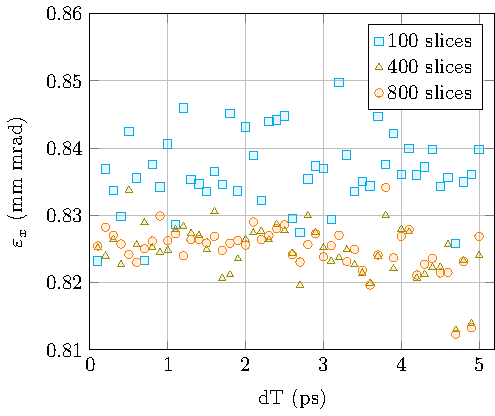
\includegraphics[width=0.8\linewidth]{Report/dt_scan}
  \caption{Envelope-tracker with different number of slices and simulation
    time steps.}
  \label{fig:et-dt}
\end{figure}

\begin{table}
  \begin{center}
    \caption{Initial conditions for the envelope tracker.}
    \label{tbl:et_params}
    \begin{tabular}{ll}
      \hline\noalign{\smallskip}
      name & initial value \\
      \noalign{\smallskip}\hline\noalign{\smallskip}
        Gun voltage       & $100$ MV\\
        %Solenoid current & $110.541$ A\\
        %Laser spot size  & $290 \times 10^{-6}$ m in x and y\\
        Bunch charge      & $200$ pC\\
        %DT$_{Gun}$        & $0.06$ ps\\
        DT$_{\text{Beamline}}$  & $1.5$ ps\\
        Number of slices  & $400$ \\
      \noalign{\smallskip}\hline
    \end{tabular}
  \end{center}
\end{table}

The parameter that affects the performance most is the number of slices.
We scanned the range from $100$ to $1000$ slices to determine the minimal
  number of slices required for stable results using various timesteps.
The results (for 100, 400 and 800 slices) of this scan are shown in
  Figure~\ref{fig:et-dt}.
Using this data we settled for $400$ slices -- increasing the slice number
  only minimally improves convergence of the results, therefore using more
  slices is inefficient.


%\begin{figure}
   %\centering
     %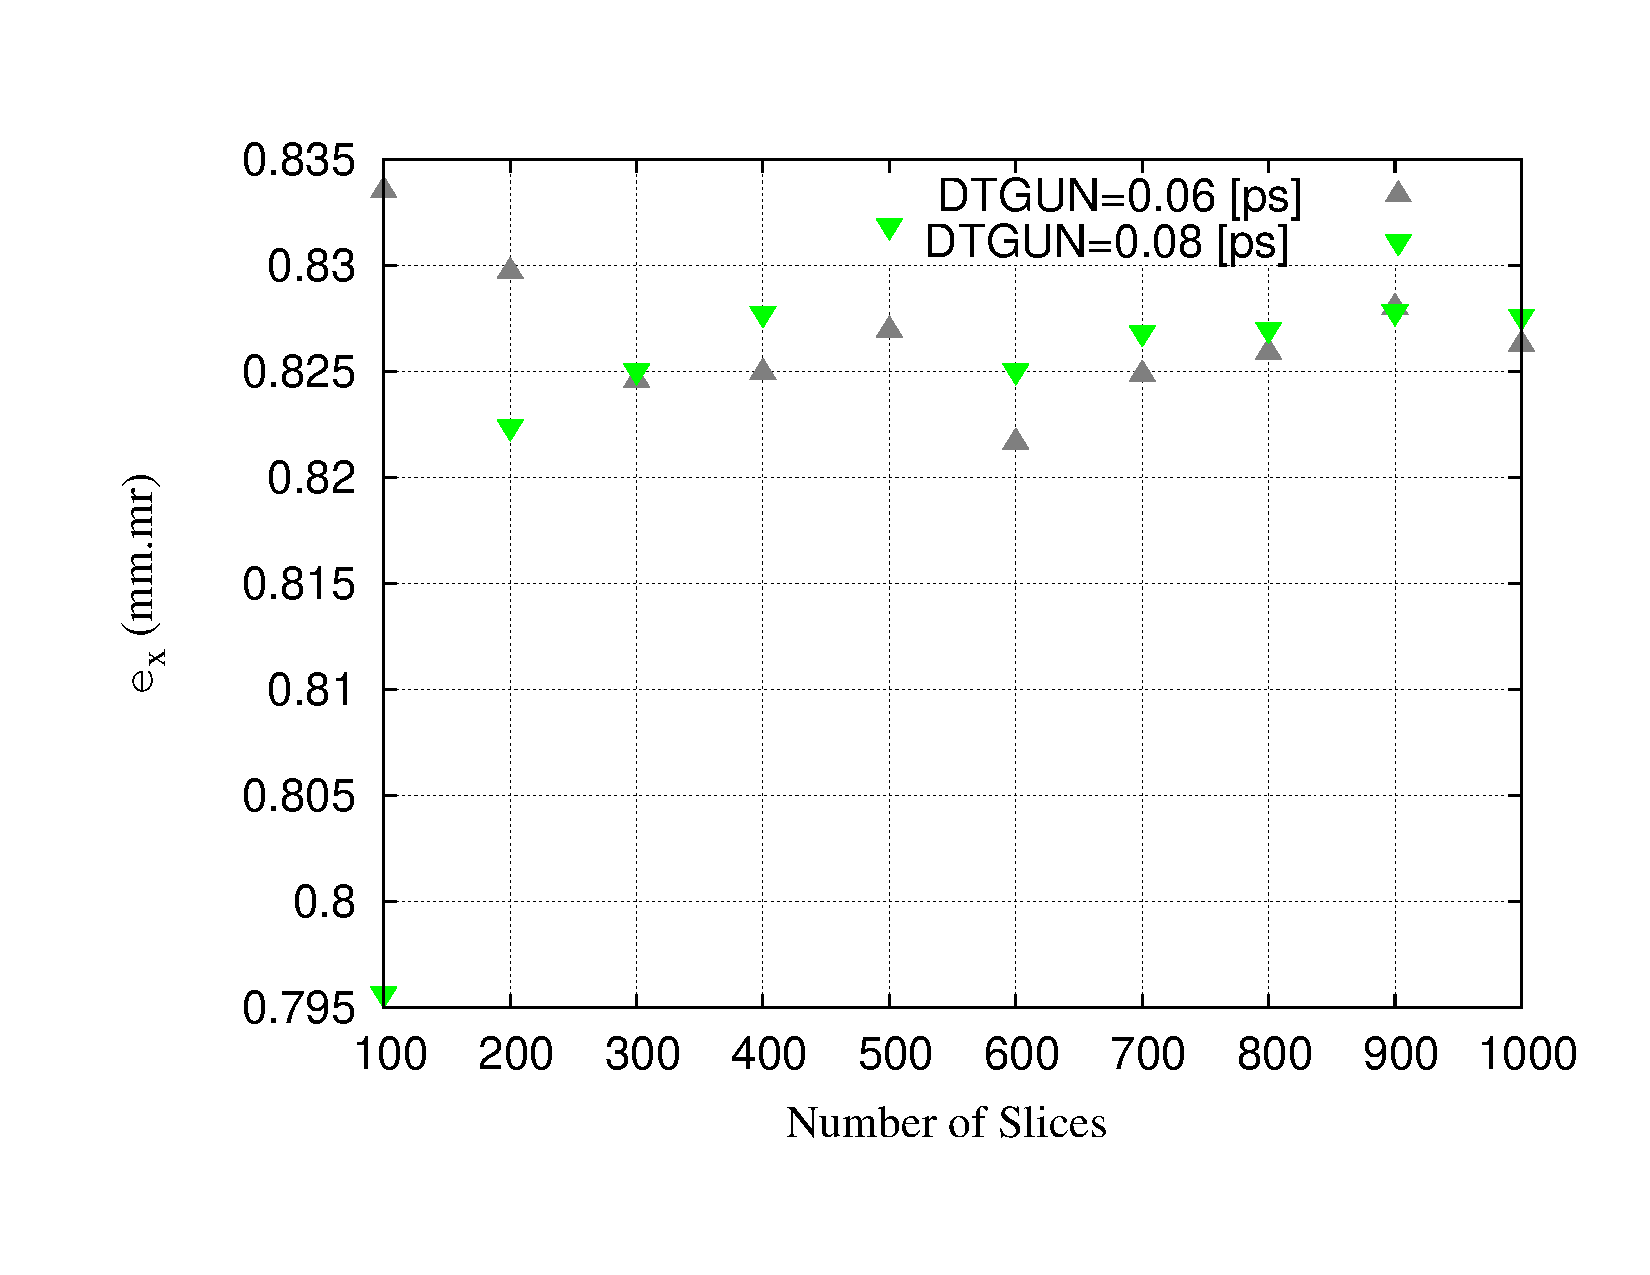
\includegraphics[angle=0,width=0.8\linewidth]{Report/sliceNew}
   %\caption{Scan of the envelope-tracker slice number showing its influence
            %on the exit emittance values.}
   %\label{fig:scan_slices}
%\end{figure}

In a next step the influence of different time steps was examined.
To that end a series of optimization runs with 100, 400 and 800 slices and
  varying timestep was performed.
%Figures \ref{fig:pareto_front_1} and \ref{fig:pareto_front_21} show two Pareto
Figure~\ref{fig:pareto_front_21} shows the Pareto fronts for 400 slices
  respectively using different timesteps.
As expected, increasing the number of slices while lowering the timestep
  produces more detailed results.

%\begin{figure}
  %\centering
    %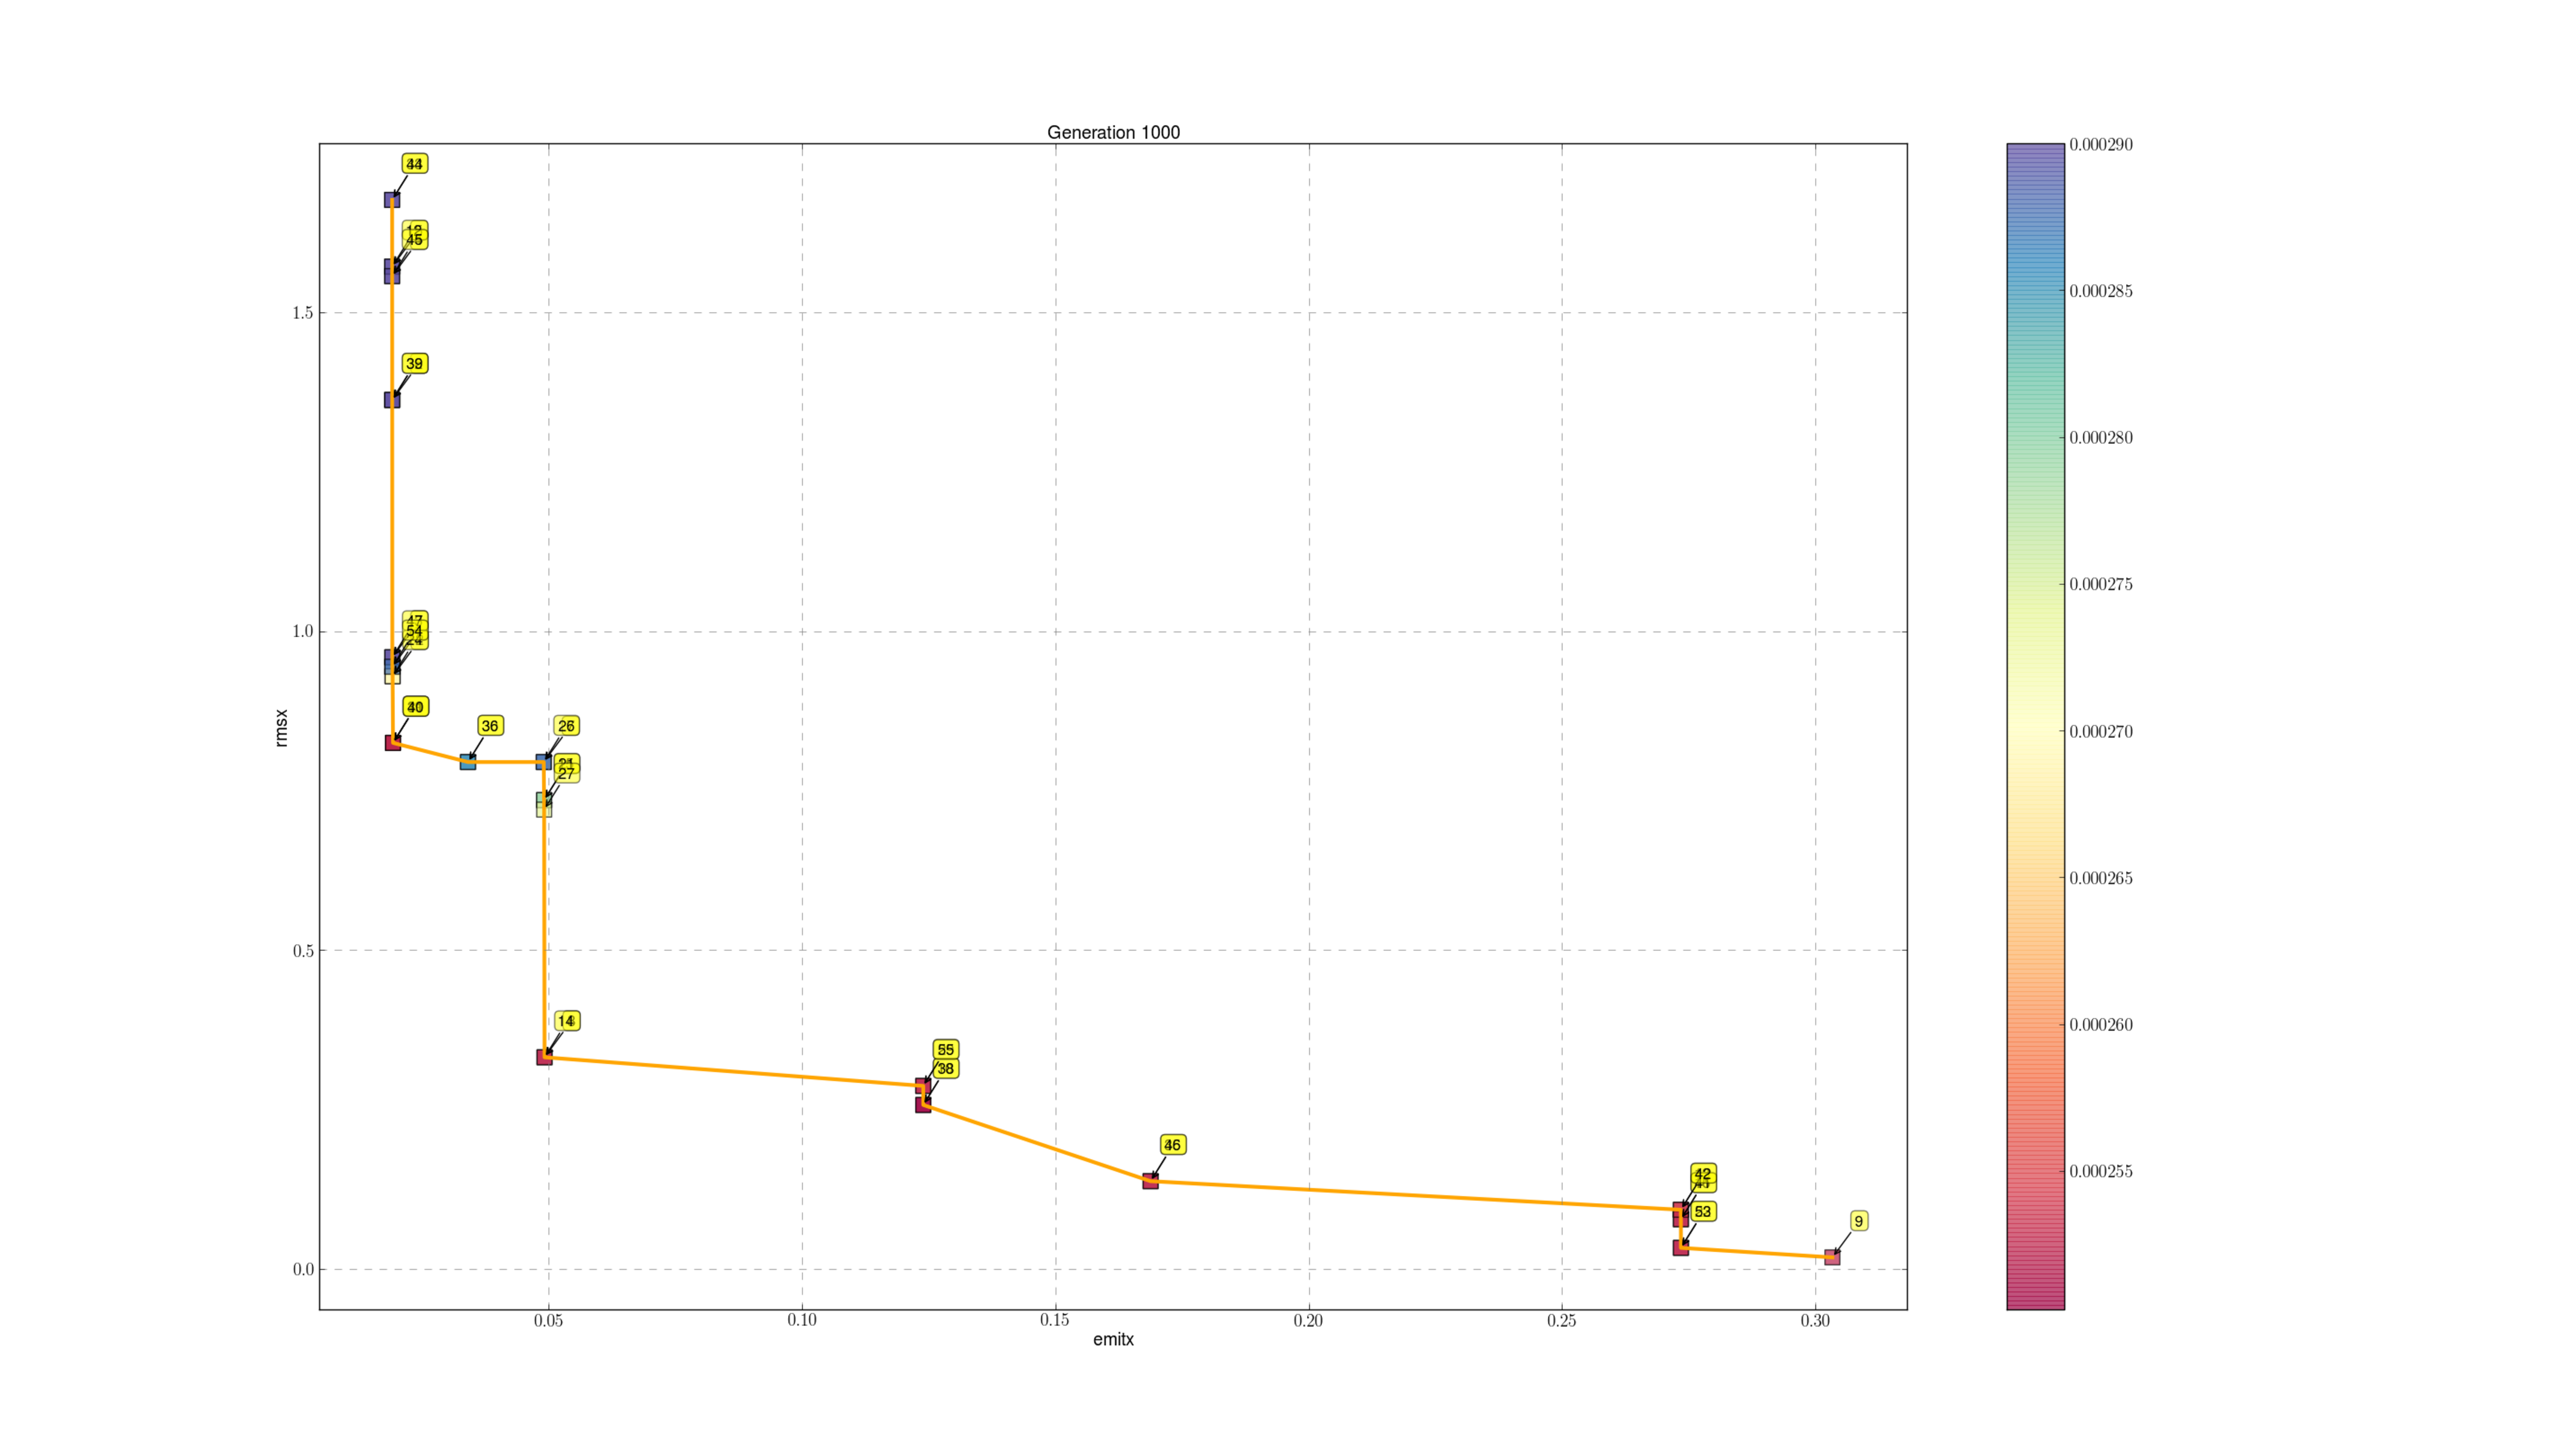
\includegraphics[width=0.9\linewidth]{Report/Run1slices100a}
  %\caption{Pareto Front for the $1000$th generation with $40$ individuals
    %using 100 slices, a simulation timestep of 5 ps and a gun timestep of 0.1
    %ps.}
  %\label{fig:pareto_front_1}
%\end{figure}

\begin{figure}%[h!]
  \centering
    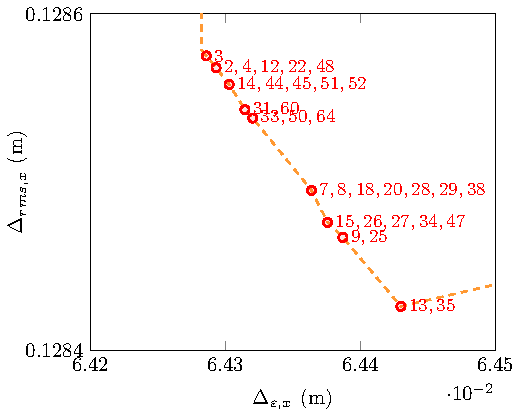
\includegraphics[width=0.8\linewidth]{Report/front_plot}
  \caption{Pareto front for the $1000$th generation with $40$ individuals
    using 400 slices (interesting region magnified), a simulation timestep
    of 1.5 ps.
    The individual 3 was selected for further investigations.}
  \label{fig:pareto_front_21}
\end{figure}


\subsubsection{Optimization Results}

Each of the $40$ points on the Pareto front, shown in
  Figure~\ref{fig:pareto_front_21}, represents an optimal solution, where
  emittance and beamsize values are compromised to achieve the best agreement
  with the Ferrario matching point.
We selected individual $3$ based on a comparison of the emittance and beamsize
  characteristics of all solutions and by retaining the feasibility of the
  beam line optics parameters.
The design variables, emittance and beamsize of the selected solution are
  shown in Table~\ref{tbl:des_vars} and Figure~\ref{fig:rmsemit}.
With the multi-objective optimization framework we attain the same working
  point as reported in~\cite{pedr:10}.

\begin{table}
  \begin{center}
    \caption{The design variables for individual $3$.}
    \label{tbl:des_vars}
    \begin{tabular}{ll}
      \hline\noalign{\smallskip}
      name & value \\
      \noalign{\smallskip}\hline\noalign{\smallskip}
        $\sigma_{x}$          & $0.262$ mm \\
        Solenoid displacement & $28.8467$ mm \\
        Gun voltage lag       & $0.0159067$ MV\\
        Solenoid current      & $111.426$ A \\
      \noalign{\smallskip}\hline
    \end{tabular}
  \end{center}
\end{table}

\begin{figure}%[h!]
  \centering
  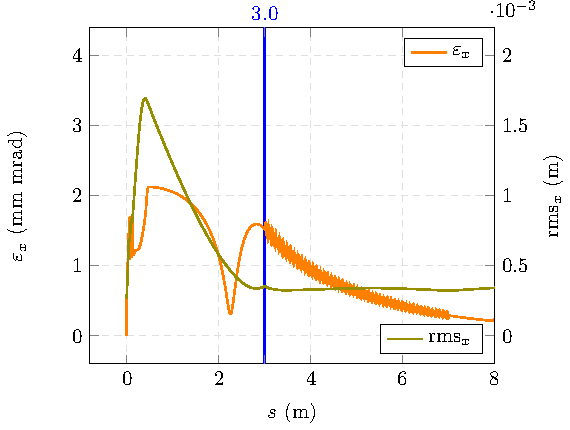
\includegraphics[width=0.8\linewidth]{Report/iff_plot_emrms}
  \caption{Beamsize and emittance of individual $3$.}
  \label{fig:rmsemit}
\end{figure}

Using the input parameters of the selected solution, we performed a stability
  analysis by varying the slice number and the time step for both the gun and
  the beam line.
Figure~\ref{fig:et-dt} shows that the exit emittance stabilizes for 400
  slices and various time steps.
No difference between $800$ and $400$ slices is visible as their minimum
  maximum extension seems to be in the same range of $0.024$ mm~mrad.

For validation purposes we compared the results of the envelope-tracker using
  the analytical space charge model with the \textsc{OPAL} 3D macro particle
  tracker.
The benchmark was run on the first 12.5 meters of the \textsc{SwissFEL} 250
  MeV injector.
The results for both rms beamsize and emittance are shown in
  Figure~\ref{fig:et-vs-tt}.
A good agreement between the two codes can be observed.
The difference of the larger emittance along the solenoids in case of 3D
  tracker that is not seen by the envelope-tracker is due to the different
  definition of the particle momenta (canonical vs.~mechanical).
Both trackers agree within acceptable limits \cite{chao:99}.

\begin{figure}
  \centering
  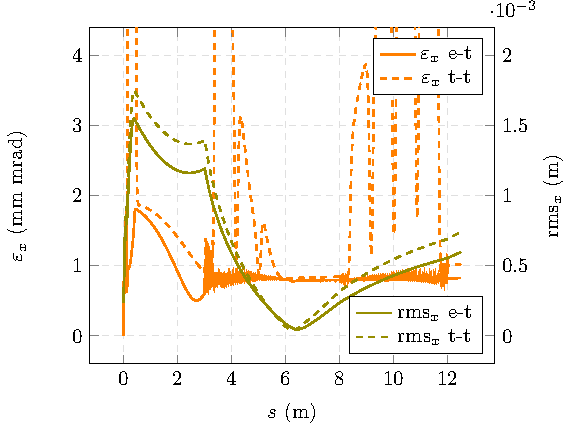
\includegraphics[width=0.9\linewidth]{Report/iff_plot_emrms_ettt}
  \caption{Comparison 3D-tracker versus envelope-tracker in case for rms$_{x}$
    and $\varepsilon_{x}$.}
  \label{fig:et-vs-tt}
\end{figure}

%\subsection{IW2: Inverse Problem}

%In order to find cross correlations we try to solve the inverse problem
  %(15) -- (23)
%%
%\begin{align}
  %\text{min}  \quad & \sqrt{\frac{1}{N} \sum \left( \text{rmx}_{x,s} -
                      %\text{m}_{x,s} \right)^2 } \text{,}\\
              %\quad & \sqrt{\frac{1}{N} \sum \left( \text{rmx}_{y,s} -
                      %\text{m}_{y,s} \right)^2 } \text{,}\\
              %\quad & \sqrt{\frac{1}{N} \sum \left( \text{rmx}_{z,s} -
                      %\text{m}_{z,s} \right)^2 } \\
  %\text{s.t.} \quad & -0.95 \leq \text{R52} \leq -0.65 \label{eq:iw2:fistdvar}\\
              %\quad & -0.90 \leq \text{R61} \leq -0.50 \\
              %\quad & 0.0   \leq \text{R62} \leq 0.20 \\
              %\quad & 0.25 \leq \text{CORR}_x \leq 0.65 \\
              %\quad & 0.55 \leq \text{CORR}_y \leq 0.95 \\
              %\quad & 0.10 \leq \text{CORR}_z \leq 0.50 \label{eq:iw2:lastdvar} \text{.}
%\end{align}
%%
%We try to match the beam to measurements from the real machine by minimizing
  %the sum of $N$ squared measurement ($m_{d,s}$ at a given position
  %$s$) errors for rmx beam size in each dimensions.
%The design variables (\ref{eq:iw2:fistdvar}) - (\ref{eq:iw2:lastdvar}) define
  %the correlation matrix used when generating particles, e.g., R51, R52, R61,
  %R62 describe limits of correlations between planes.
%The initial Binomial distribution (with $m = ?$) has the form
%%
%\begin{equation*}
  %\frac{1}{2\pi\sigma_x\sigma_y}exp(-\frac{x^2}{2\sigma_x^2}
  %-\frac{y^2}{2\sigma_y^2})
  %\text{.}
%\end{equation*}
%%

%Since these correlations cannot be measured we get the real values by solving
  %the inverse problem mentioned above.

%Currently we run the simulations on a low resolution space charge grid ($8
  %\times 8 \times 8$) as a proof of concept.
%In a next step a simple Python script would be applied to iteratively rerun
  %the optimizer with increasing space-charge resolution when the limits of the
  %design variables are narrow enough (iteratively diminishing search space).
%\subsection{IW2: Inverse Problem}

%In order to find cross correlations we try to solve the inverse problem
  %(15) -- (23)
%%
%\begin{align}
  %\text{min}  \quad & \sqrt{\frac{1}{N} \sum \left( \text{rmx}_{x,s} -
                      %\text{m}_{x,s} \right)^2 } \text{,}\\
              %\quad & \sqrt{\frac{1}{N} \sum \left( \text{rmx}_{y,s} -
                      %\text{m}_{y,s} \right)^2 } \text{,}\\
              %\quad & \sqrt{\frac{1}{N} \sum \left( \text{rmx}_{z,s} -
                      %\text{m}_{z,s} \right)^2 } \\
  %\text{s.t.} \quad & -0.95 \leq \text{R52} \leq -0.65 \label{eq:iw2:fistdvar}\\
              %\quad & -0.90 \leq \text{R61} \leq -0.50 \\
              %\quad & 0.0   \leq \text{R62} \leq 0.20 \\
              %\quad & 0.25 \leq \text{CORR}_x \leq 0.65 \\
              %\quad & 0.55 \leq \text{CORR}_y \leq 0.95 \\
              %\quad & 0.10 \leq \text{CORR}_z \leq 0.50 \label{eq:iw2:lastdvar} \text{.}
%\end{align}
%%
%We try to match the beam to measurements from the real machine by minimizing
  %the sum of $N$ squared measurement ($m_{d,s}$ at a given position
  %$s$) errors for rmx beam size in each dimensions.
%The design variables (\ref{eq:iw2:fistdvar}) - (\ref{eq:iw2:lastdvar}) define
  %the correlation matrix used when generating particles, e.g., R51, R52, R61,
  %R62 describe limits of correlations between planes.
%The initial Binomial distribution (with $m = ?$) has the form
%%
%\begin{equation*}
  %\frac{1}{2\pi\sigma_x\sigma_y}exp(-\frac{x^2}{2\sigma_x^2}
  %-\frac{y^2}{2\sigma_y^2})
  %\text{.}
%\end{equation*}
%%

%Since these correlations cannot be measured we get the real values by solving
  %the inverse problem mentioned above.

%Currently we run the simulations on a low resolution space charge grid ($8
  %\times 8 \times 8$) as a proof of concept.
%In a next step a simple Python script would be applied to iteratively rerun
  %the optimizer with increasing space-charge resolution when the limits of the
  %design variables are narrow enough (iteratively diminishing search space). 
%\vspace{-7em}
\subsection{AWA Photoinjector Optimization} \label{awaproblem}
Next we apply the optimization framework to the high charge beam line at the AWA. 
The purpose of the Argonne Wakefield Accelerator (AWA) optimization is to produce beams of electrons meeting 
design specifications including number of particles (charge), energy, and particle distribution (characterized by transverse beam sizes and energy spread).
As shown in Fig.  \ref{awa-pic}, this beam line consists of an rf photocathode gun, 
two solenoids, six linear accelerating cavities, 
followed by four quadrupoles and a stripline kicker. 
The charge of interest, 40 nC, is needed for Two Beam 
Acceleration (TBA) \cite{gai_power_jing_2012} experiments performed in the past 
at AWA. Similar experiments will take place in the future and motivate this work. 
Prior experimental results were limited by beam size as the beam passed through small aperture 
wakefield structures located after the quadrupoles. 
In an attempt to maximize charge transmission in upcoming experiments
we optimize several parameters in the gun and quadrupoles leading into the 
TBA section of the beam line.
%\vspace{-1em}

\begin{figure}
	\begin{tikzpicture}[every node/.style={anchor=south west,inner sep=0pt},x=1mm, y=1mm,]   
	\node (fig1) at (0,0)
	{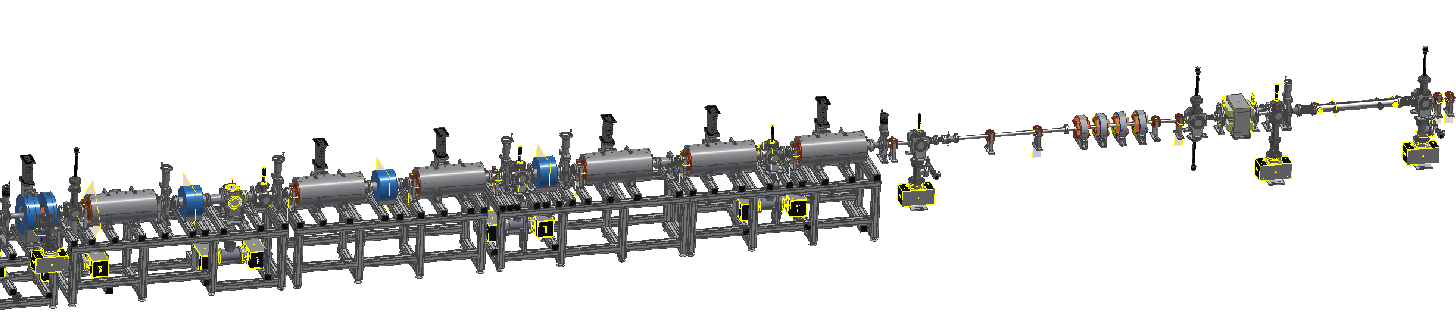
\includegraphics[width=\textwidth]{Report/awa-drawing}};
	\node[fill=white, inner sep=2pt] (txt2) at (125,10) {$s_2$};
	\node[fill=white, inner sep=2pt] (txt2) at (112,8) {$s_1$};
	\node[fill=white, inner sep=2pt] (txt2) at (115,30) {Kicker};
	\draw [blue, ->, line width=1] (120,30) -- (120, 23);	
	\end{tikzpicture}
	\caption{Side view of the high charge linac at the AWA. 
		All hardware in this drawing is currently installed.}
	\label{awa-linac}
\end{figure}

\begin{figure}
	\begin{tikzpicture}[every node/.style={anchor=south west,inner sep=0pt},x=1mm, y=1mm,]   
	\node (fig2) at (0,0)
	{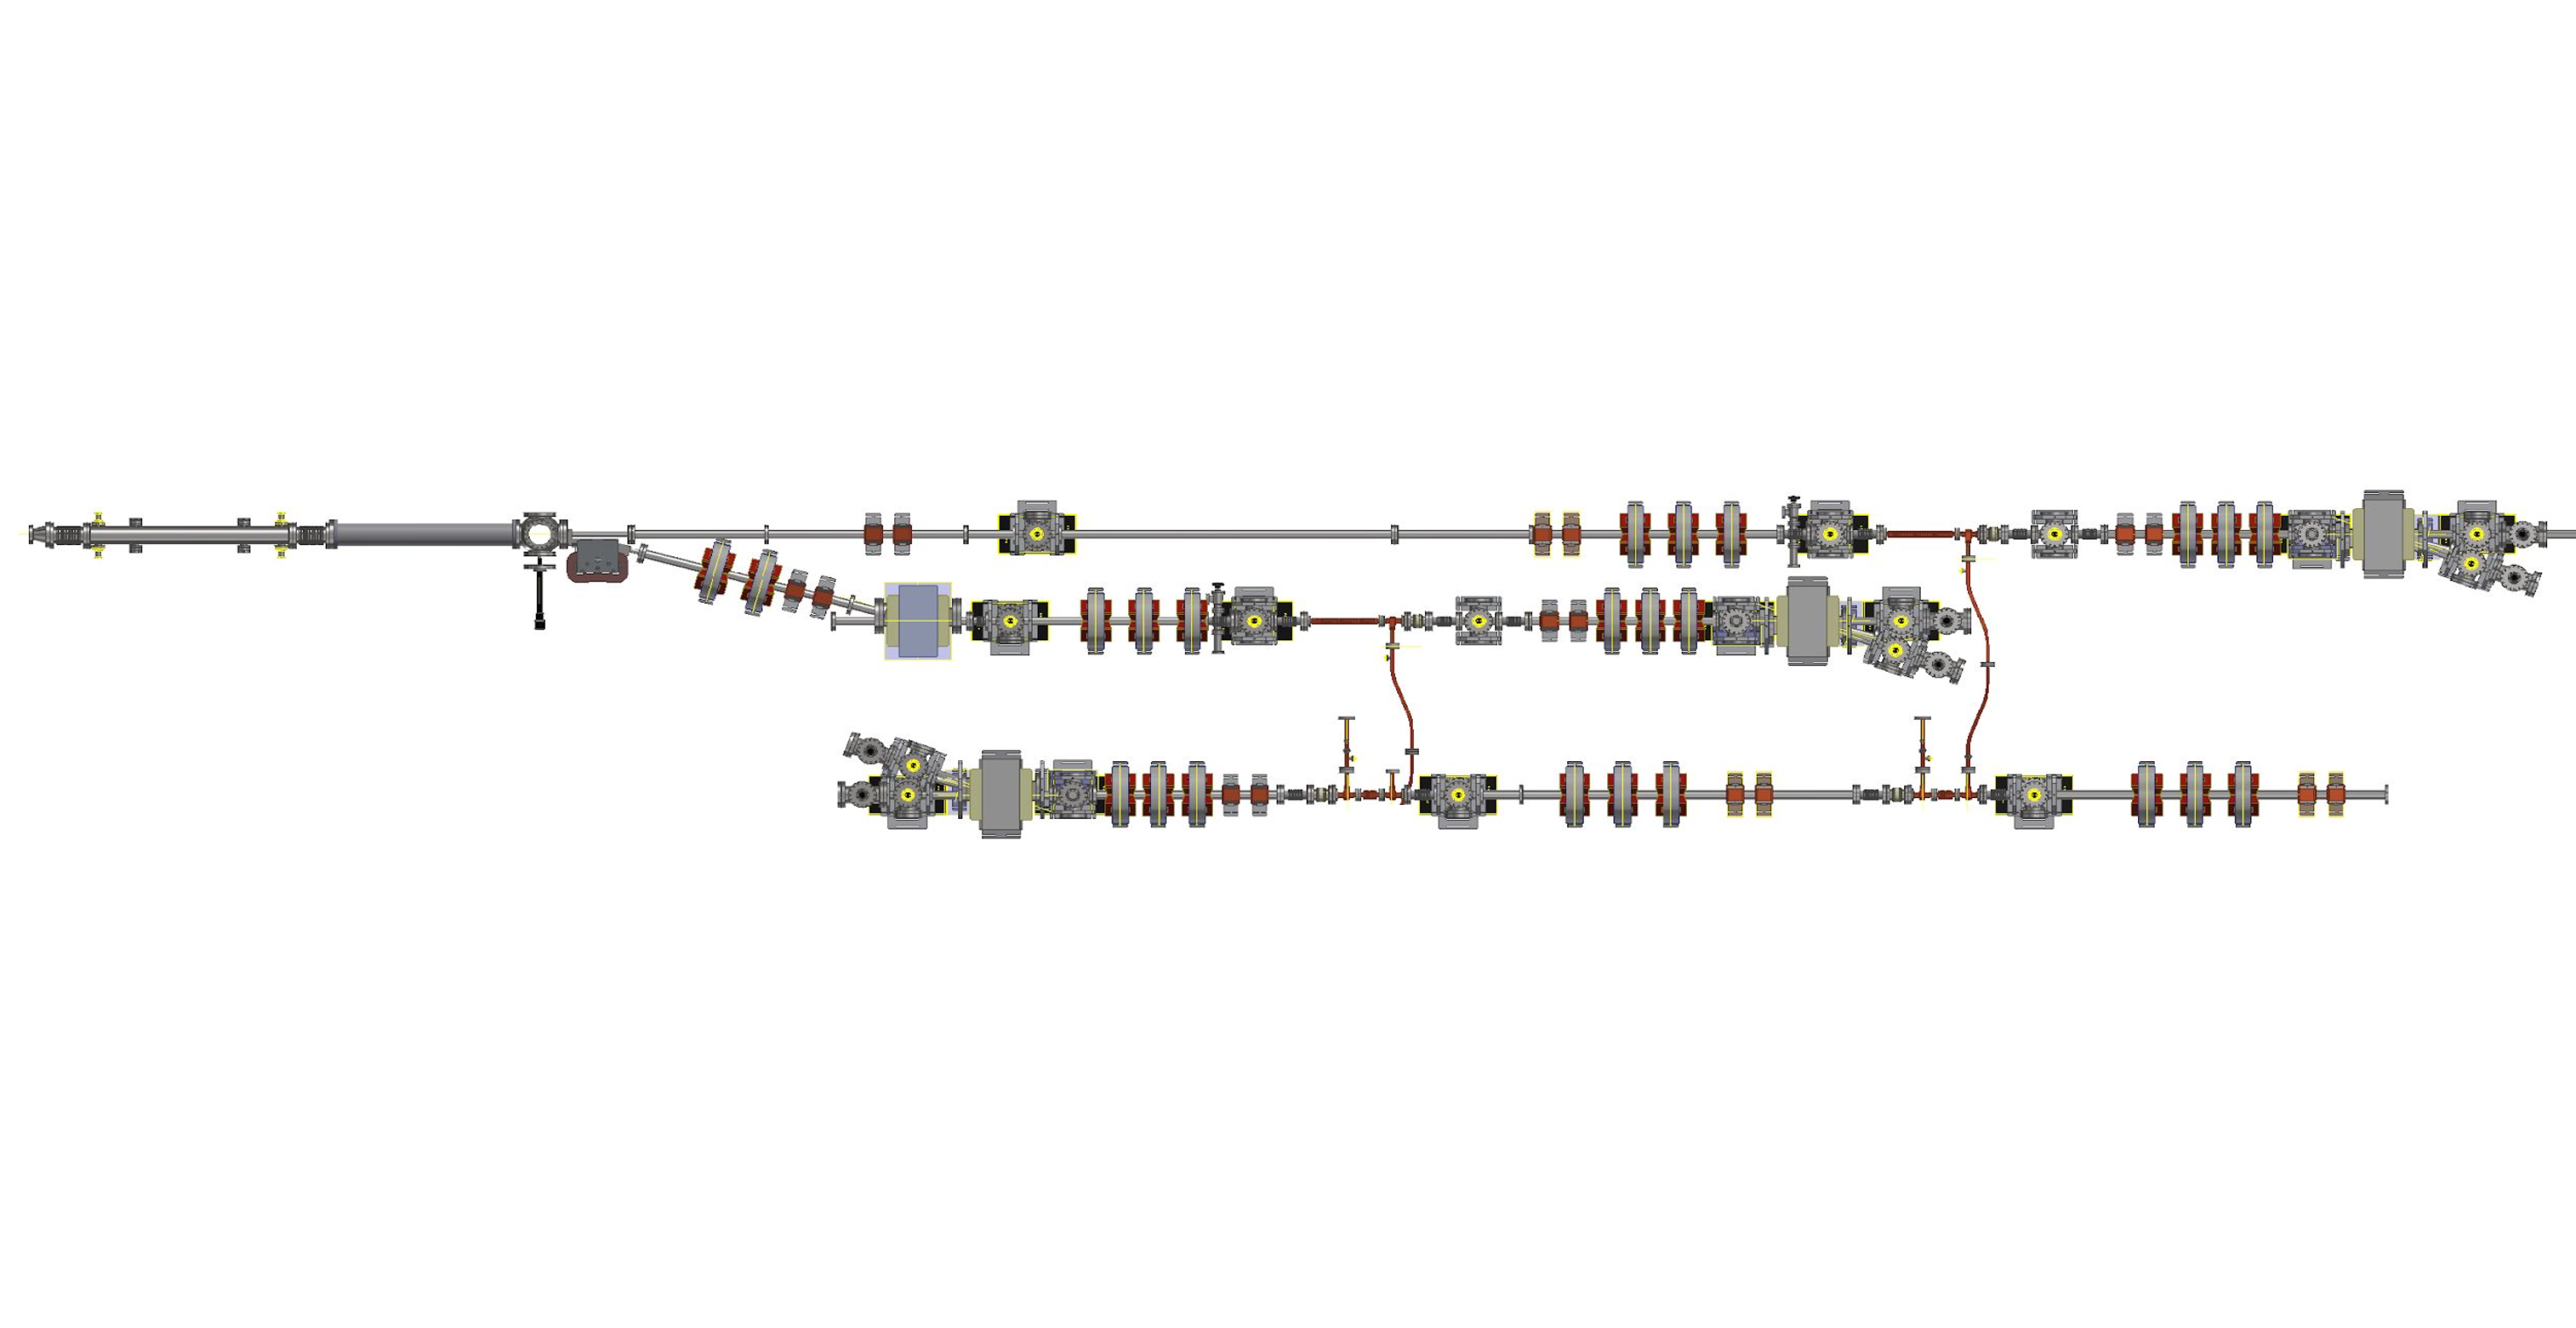
\includegraphics[width=\textwidth]{Report/tba_dogleg}};
	\node[fill=white, inner sep=2pt] (txt2) at (2,35) {$s_1$};
	\node[fill=white, inner sep=2pt] (txt2) at (14,35) {$s_2$};
	\node[fill=white, inner sep=2pt] (txt2) at (33,31) {$s_3$};
	\node[fill=white, inner sep=2pt] (txt2) at (24,50) {Septum};
	\draw [blue, ->, line width=1] (30,50) -- (30, 42);	
	\node[fill=white, inner sep=2pt] (txt2) at (3,50) {Kicker};
	\draw [blue, ->, line width=1] (9.5,50) -- (9.5, 43);
	\end{tikzpicture}
	\caption{Continuation of the high charge beam line layout at the AWA, top view. 
		This is the proposed two beam acceleration section.}
	\label{awa-tba}
\end{figure}

%\vspace{-1em}
In addition to the physics challenges, we chose this model to demonstrate the ability of the framework to tackle large problems.
Six design variables and objectives were used, 
along with three constraints.
The objectives include transverse and longitudinal beam size, 
transverse momentum and longitudinal energy spread. 
The design variables include the two gun solenoids and 
the first four quadrupoles. The objectives are calculated at 
$s_1=19.4$~[m], at the entrance of the fifth quadrupole in Fig.~\ref{awa-pic}.  
This problem encompasses high dimensionality 
and nonlinear effects such as space charge. There is no existing information
that accurately predicts where the Pareto front will fall. This work is also meaningful in that
it will guide future operations at the AWA.
\nrnote{Maybe eqs 5.10-5.21 and code example should move after time step scan and hyper parameters}

\begin{align}
\text{min}  \quad & \text{rms}_{x}\left(s = s_3\right), \quad \text{rms}_{y}\left(s = s_3\right) \label{eq:awa:p1}\\
& \text{rms}_{px}\left(s = s_3\right), \quad \text{rms}_{py}\left(s = s_3\right), \label{eq:awa:p2}\\
& \text{rms}_{s}\left(s = s_3\right), \quad dE \label{eq:awa:p4} \\
\text{subject to} \quad & rms_x(s=s_1) < 0.1 \, [m]\label{eq:awa:c1}\\
\quad & rms_y(s=s_1) < 0.1\, [m]\label{eq:awa:c2}\\
\quad & |rms_y(s=s_1) - rms_x(s=s_1) | < 0.005 \, [m]\label{eq:awa:c3}\\
\quad & q = 40 \left[\text{nC}\right] \label{eq:awa:firstconstr}\\
\quad & \text{Volt}_{\text{Gun}} = 64\left[\text{MV/m}\right] \label{eq:awa:lastconstr}\\
\quad & \text{Volt}_{\text{Linac}} = 24-25\left[\text{MV/m}\right] \\
\quad & R_x = R_y = 9 \left[\text{mm}\right] \label{eq:awa:firstdvar}\\
\quad & \phi_{\text{gun}} =-20^\circ \label{eq:awa:gphidvar}\\
\quad & \phi_{\text{linac}} =-20^\circ \label{eq:awa:lastdvar}
\end{align}

The first four objectives, Eqs. (\ref{eq:awa:p1}) to (\ref{eq:awa:p2}),
minimize the transverse ($rms_{x,y}$) beam size and transverse momentum ($rms_{px,py}$)
at the location of interest in the beam line ($s_1$).
Where $s_1$ is the longitudinal entrance of the fifth quadrupole. 
Minimizing the beam size at this location is essential to 
to preventing loss of particles by scraping.
Preventing scraping ensures better transmission through the wakefield structures downstream. 
Less divergence in the beam (lower transverse momentum) 
reduces growth of transverse beam size during transport in bending elements, 
which also helps with transmission downstream. 
The next two objectives (\ref{eq:awa:p2}) minimize the 
longitudinal beam size ($rms_s$), and energy spread (dE) at $s_1$.
This helps reduce longitudinal beam size growth in bending elements.  

Three constraints were also defined to help guide the algorithm;
Eqs.~\ref{eq:awa:c1} to \ref{eq:awa:c3}.
The bounding values may seem large, but this is done to avoid over constraing the 
problem in early generations. If the constraints are set tighter, 
runs do not reach the second generation, because enough satisfactory 
points are not produced to fill a complete generation. 
Leaving the value large allows for enough simulations to finish
in order to reach the next generation, and subsequent improved points in later generations.
The difference constraint, Eq.~\ref{eq:awa:c3}, is used to favor nearly round beams.
This prevents one dimension from becoming disproportionately large compared to the other.
In this case, there is some room in the beam pipe to allow the y dimension to grow, but round beams 
are preferred for easier data analysis.

Equations (\ref{eq:awa:firstconstr}) to
(\ref{eq:awa:lastdvar}) define the charge, gun voltage, linac voltages, 
laser radius, gun phase, and linac cavity phases (in that order). 
These are parameters in the simulation 
that must be defined, but do not vary during the optimization.
%\vspace{-1em}
As introduced in Section \ref{ferrario}, we define the AWA optimization 
design variables, objectives, and constraints in the OPAL input file as shown in
the following code: %equations (\ref{eq:awa:p1}) to (\ref{eq:awa:lastdvar}). 

\vspace{0.2cm}
{\footnotesize \begin{verbatim}
	
	// Gun variables 
	dv0: DVAR, VARIABLE="IBF",    LOWERBOUND=300.0, UPPERBOUND=500.0;
	dv1: DVAR, VARIABLE="IM",     LOWERBOUND=180.0, UPPERBOUND=280.0;
	
	// Quad variables 
	dv4: DVAR, VARIABLE="KQ1", LOWERBOUND=-8.0, UPPERBOUND=8.0;
	dv5: DVAR, VARIABLE="KQ2", LOWERBOUND=-8.0, UPPERBOUND=8.0;
	dv6: DVAR, VARIABLE="KQ3", LOWERBOUND=-8.0, UPPERBOUND=8.0;
	dv7: DVAR, VARIABLE="KQ4", LOWERBOUND=-8.0, UPPERBOUND=8.0;
	
	//Objectives
	de3: OBJECTIVE,EXPR="fabs(statVariableAt('dE',19.4))";
	rmss3: OBJECTIVE,EXPR="fabs(statVariableAt('rms_s',19.4))";
	rmsx3: OBJECTIVE,EXPR="fabs(statVariableAt('rms_x',19.4))";
	rmsy3: OBJECTIVE,EXPR="fabs(statVariableAt('rms_y',19.4))";
	rmspx3: OBJECTIVE,EXPR="fabs(statVariableAt('rms_px',19.4))";
	rmspy3: OBJECTIVE,EXPR="fabs(statVariableAt('rms_py',19.4))";
	
	//Kicker apeture
	c1: CONSTRAINT, EXPR="fabs(statVariableAt('rms_x',16.5))<0.1";
	c2: CONSTRAINT, EXPR="fabs(statVariableAt('rms_y',16.5))<0.1";
	c3: CONSTRAINT, EXPR="fabs(statVariableAt('rms_y',16.5)-statVariableAt('rms_x',16.5))<0.005";
	
	OPTIMIZE, INPUT="tmpl/optLinac-40nC.tmpl",
	OUTPUT="optLinac-40nC",
	OUTDIR="results",
	OBJECTIVES = {rmss3, rmsx3, rmsy3, rmspx3, rmspy3, de3},
	DVARS = {dv0, dv1, dv4, dv5, dv6, dv7},
	CONSTRAINTS = {c1, c2, c3},
	INITIALPOPULATION=656,
	MAXGENERATIONS=200,
	NUM_MASTERS=1,
	NUM_COWORKERS=8,
	SIMTMPDIR="tmp",
	TEMPLATEDIR="tmpl",
	FIELDMAPDIR="fieldmaps",
	NUM_IND_GEN=328,
	GENE_MUTATION_PROBABILITY=0.01,
	MUTATION_PROBABILITY=0.01,
	RECOMBINATION_PROBABILITY=0.09;
	QUIT;
	
	\end{verbatim}}
\vspace{0.2cm}

Design variables include the currents in two gun solenoids (IBF and IM), 
and four quadrupole strengths (KQ1-KQ2). The objectives include
beam size (transverse and longitudinal), transverse momentum, and energy spread as
defined in Eqs. (\ref{eq:awa:p1}) to (\ref{eq:awa:p4}). 
The location at the entrance of the kicker is $s_0=16.45$~meters, 
and the location of interest for objectives is $s_1=19.4$~meters. 

All simulations for this experiment were carried out on Bebop a
high performance computing (HPC)
cluster provided by the Laboratory Computing Resource Center (LCRC)
at Argonne National Laboratory (ANL). We used Intel Knights Landing 
(KNL) processors at 1.3 GHz with 128 GB of memory 
and 64 cores per node. There are 352 compute nodes available on 
Bebop, with a total of 22,528 cores. All jobs were run and compared 
on 8 cores each, which allowed 8 jobs per node on the KNLs.
This in combination with the number of nodes available 
allows for very large optimization jobs, like the AWA case.
Typical runs for this paper used 41 nodes, which corresponds to 2624 KNL cores 
and a generation size of 328 individuals.



\subsubsection{Time Step Scan} \label{awa:subsection:test}
A study on time step and 
number of particles was done to reduce the time to simulation while 
maintaining the physics of interest. 
The grid size $16 \times 16 \times 32$ was chosen, 
and parallelized in the x and y directions.
After comparing several options we choose ten thousand particles 
in combination with adjusting the time step (dT) near sensitive elements 
(i.e. quadurpoles, kicker). 
The resulting simulations are low fidelity, but closely approximate 
the mid fidelity simulations for metrics of interest, as shown in 
Fig. \ref{tstep}. For all models, the longitudinal parameters (rms$_s$ and energy) 
are calculated correctly, but we see discrepancies in the transverse 
rms$_x$ and $\epsilon_x$ in the low fidelity results. The
average run time of each simulation with the adjusted time steps was 1.6~minutes.
In comparison the mid fidelity simulations ran for 18~minutes.
%A summary of the parameters used is listed in Table \ref{fidelity}. 

\begin{figure}
	\centering
	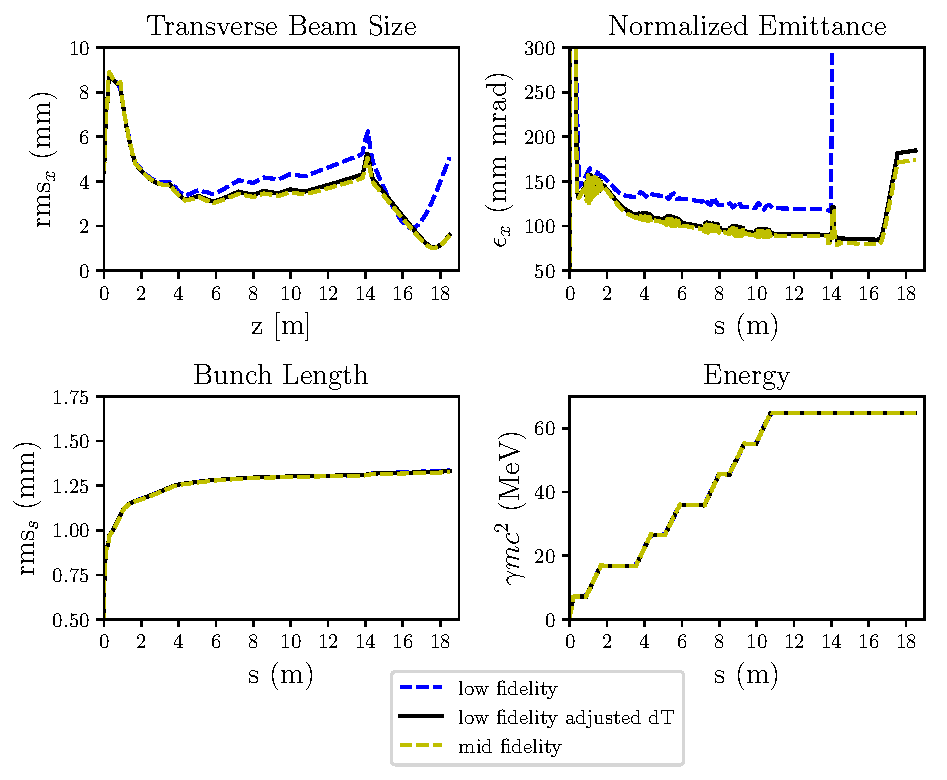
\includegraphics[width=0.8\linewidth]{Report/timestep_comparison}
	\caption{Comparison of different fidelity models (dT stands for time step).}
	\label{tstep}
\end{figure}

\iffalse
\begin{table}%[h!]
	\begin{center}
		\caption{Low and mid fidelity simulation parameters.}
		\label{fidelity}
		\begin{tabular*}{\textwidth}{l @{\extracolsep{\fill}} C c D }
			\hline\noalign{\smallskip}
			& Number of particles & dT (seconds) & Time to simulation (minutes)\\
			\noalign{\smallskip}\hline\noalign{\smallskip}
			low fidelity  			&  10,000   & $5 \times10^{-11}$  &  2.6 \\
			adjusted low fidelity  	&  10,000   & $2 \times 10^{-12}$, $1 \times 10^{-11}$ & 1.6 \\
			mid fidelity 			&  100,000  & $1 \times 10^{-12}$ &  18\\
			\noalign{\smallskip}\hline
		\end{tabular*}
	\end{center}
\end{table}
\fi 

\subsubsection{Hyper parameter Scan}
While the optimization problem and goals were well defined (Section \ref{awaproblem}), 
it was not clear what the best input parameters for the NSGA-II should be.
These parameters include gene mutation probability, mutation probability, 
recombination probability, number of individuals, 
and number of generations to complete. 
Given the beam line and design variables given in Section \ref{awaproblem},
\nrnote{Changed variables for final run, the variables in 5.3 no longer match these small runs. Need to rework this section} 
four optimization experiments were done with varying NSGA-II parameters. 
Similar to the time step scan, 
the goal of this exercise was to determine which set of optimization
parameters strongly influence the results, 
and whether there was a time to solution difference.
From here on, we will reference each experiment as ex-1, ex-2, ex-3, and ex-4
as shown in Table \ref{extable}. 
\begin{table}%[h!]
	\begin{center}
		\caption{Input Parameters for initial twenty four hour AWA optimization experiments. 
			The gene mutation probability was equal to the mutation probability (not shown) in all four experiments. 
			The max number of individuals per generation was~80.}
		\label{extable}
		\begin{tabular*}{\textwidth}{l @{\extracolsep{\fill}} C C D }
			\hline\noalign{\smallskip}
			& Gene Mutation Probability & Recombination Probibility & Number of completed generations \\
			\noalign{\smallskip}\hline\noalign{\smallskip}
			ex-1 &  0.1  & 0.9  &  96 \\
			ex-2 &  0.3  & 0.7  &  81 \\
			ex-3 &  0.8  & 0.2  &  53 \\
			ex-4 &  0.01 & 0.09 &  95 \\
			\noalign{\smallskip}\hline
		\end{tabular*}
	\end{center}
\end{table}


The maximum number of individuals per generation was fixed at 80, 
Each experiment was allowed to run for twenty four hours, with 
a maximum generation limit of 100. 
We reduced the seven objectives to the four needed to construct 
the Pareto fronts that would be the final goal of this study.
The objectives include: $\varepsilon_{x}\left(s = s_1\right)\text{, } \varepsilon_{x}\left(s = s_2\right)\text{, } \text{rms}_{s}\left(s = s_1\right)\text{, and }  \text{rms}_{s}\left(s = s_2\right)$. 
\lsnote{You could define $\varepsilon_{x1}$ to be $\varepsilon_{x} (s=s1)$ and similarly in the table and then use going forward to simplify notation}
The optimization parameters specific to OPAL input for ex-3 are given as an example.
Note the design variables defined in Section \ref{awaproblem}
precede the optimization parameters in the OPAL input file.

\vspace{0.2cm}
{\footnotesize \begin{verbatim}
	OPTIMIZE, INPUT="tmpl/optLinac_40nC.tmpl",
	OUTPUT="optLinac_40nC",
	OUTDIR="results",
	OBJECTIVES = {rmss1, rmsx1, emitx1, de1, rmss2, rmsx2, emitx2},
	DVARS = {dv0, dv1, dv2, dv3, dv4, dv5, dv6, dv7},
	CONSTRAINTS = {c1, c2},
	INITIALPOPULATION=656,
	MAXGENERATIONS=200,
	NUM_MASTERS=1,
	NUM_COWORKERS=8,
	SIMTMPDIR="tmp",
	TEMPLATEDIR="tmpl",
	FIELDMAPDIR="fieldmaps",
	NUM_IND_GEN=328,
	GENE_MUTATION_PROBABILITY=0.8,
	MUTATION_PROBABILITY=0.8,
	RECOMBINATION_PROBABILITY=0.2;
	QUIT;
	\end{verbatim}}
\vspace{0.2cm}

After collection of the data for all four experiments, several metrics
were compared, including number of generations completed in twenty four hours,
Pareto fronts at $s_1$ and $s_2$, and the design variables at the Pareto front. 
From Table \ref{extable}, we clearly see ex-3 is significantly 
slower, as it evaluated about 30 to 40 fewer generations than the other experiments.
Perhaps this trade off would be acceptable if the Pareto front was significantly 
improved, but from Fig. \ref{expareto}, we can see this is not the case.
The Pareto fronts at $s_1$, are nearly identical. We could expect
they would continue to converge given more time. 
Similar arguments can be made for ex-2, which evaluated about 15 less generations
with no clear benefit in either Pareto front.
When looking at the Pareto front at $s_2$, only ex-4 has a slight 
edge over the others.
With ex-2 and ex-3 eliminated due to evaluation time, 
the hyper parameters in ex-4 were chosen as the default values for subsequent runs.
\iffalse  
\begin{figure}
	\centering
	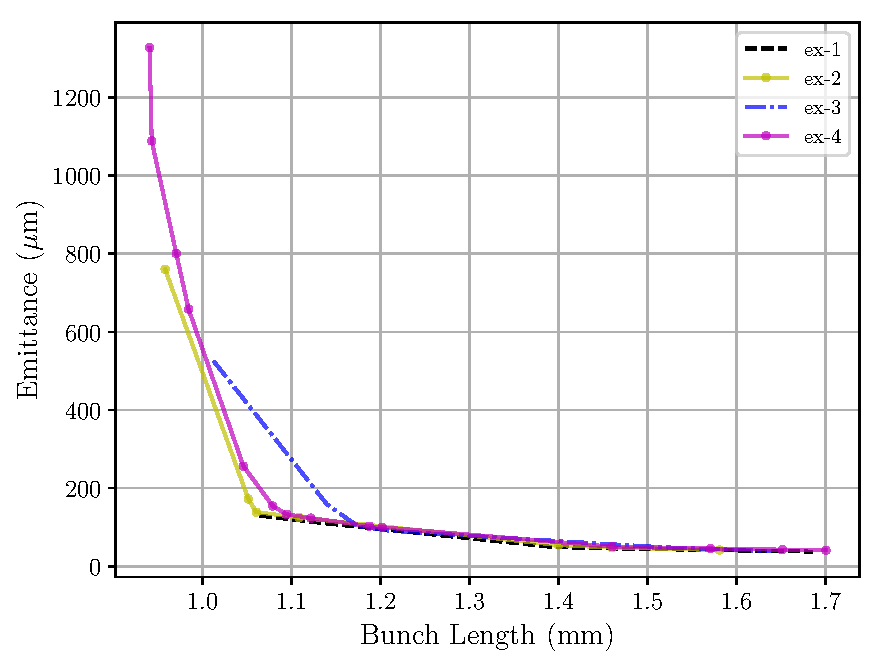
\includegraphics[width=0.75\textwidth]{Report/ex-pareto1}%
	\llap{\raisebox{1.8cm}{%  move next graphics to top right corner
			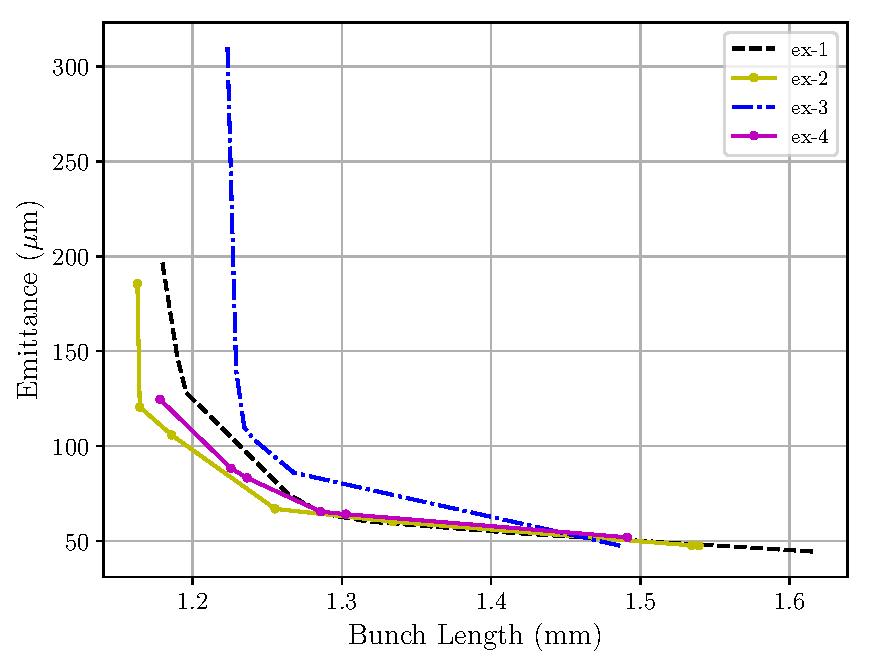
\includegraphics[height=5.5cm]{Report/ex-pareto2}%
	}}
	\caption{My overlay figure.}
\end{figure}  
\fi

\begin{figure}
	\centering
	\begin{subfigure}{0.49\textwidth}
		\centering
		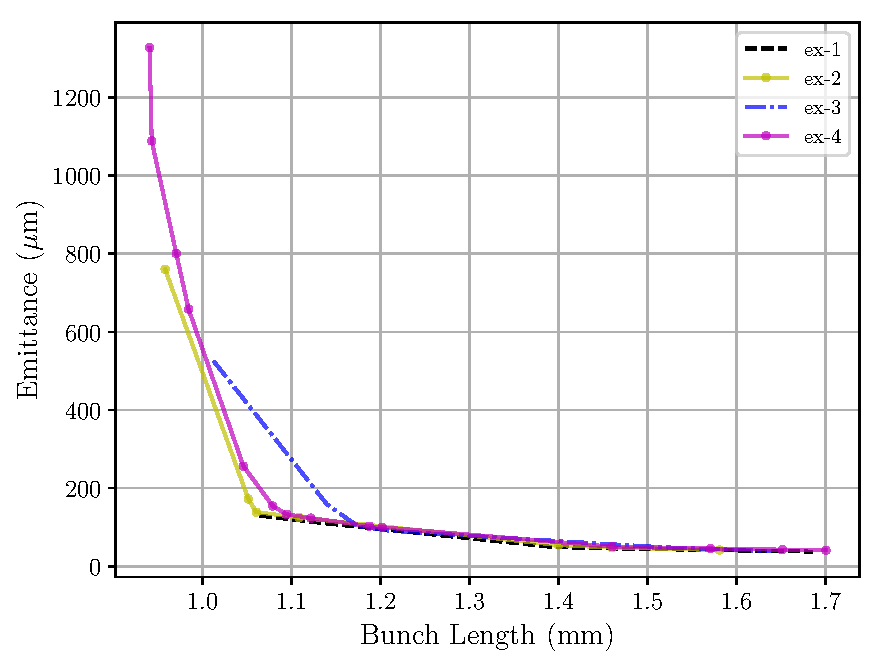
\includegraphics[width=\textwidth]{Report/ex-pareto1}
		\caption{Pareto fronts at $s_1$.}
		\label{expareto1}
	\end{subfigure}
	\begin{subfigure}{0.49\textwidth}
	\centering
	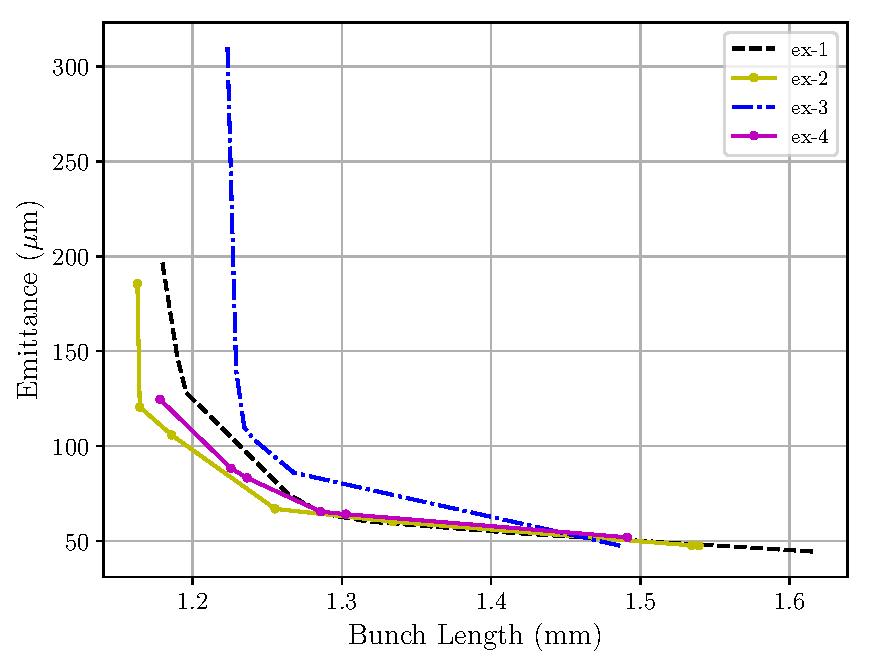
\includegraphics[width=\textwidth]{Report/ex-pareto2}
	\caption{Pareto fronts at $s_2$.}
	\label{expareto2}
	\end{subfigure}
	\caption{Comparison of Pareto fronts for initial optimization experiments.}
	\label{expareto}
\end{figure}
 


\subsubsection{AWA Optimization Results}
With the time steps and hyper parameters set by the work in \ref{awa:subsection:test}, 
the full optimization problem described in \ref{awaproblem} was run for 200 generations.
The initial number of individuals was fixed at 656, 
and the minimum number individuals in later generations was fixed at 328. 
These numbers were in part based on the architecture of the KNL's. 
Since each simulation takes 8 cores, and there are 64 cores per KNL node, 
we wanted a large population size that would fit evenly on these resources. 

Again, the location of optimization is $s_3=19.4$ [m]. 
This is the entrance to the fifth quad in the beam line. 
This location is where the beam should be captured and focused through subsequent elements.
After collection of the data, Pareto fronts comparing the objectives were plotted, 
see Figs. X-Z.
The $\sigma_x$ and $\sigma_{px}$ plots are of most interest, as they are the most heavility 
impacted by bending elements. With this in mind, several beam parameters corresponding to
options on Pareto Front in Fig. X were plotted and compared. 
The best results are shown in Fig. Z. 
The maximum beam sizes are well below the beam pip aperture limits as shown in Fig. (b). 
 
\begin{figure}
	%\includegraphics[width=0.5\textwidth]{}\includegraphics[width=0.5\textwidth]{}
	\label{beamsizes}
\end{figure}







